\section{Introduction}

The cerebellum is a fundamental structure of the hindbrain, and it is responsible of coordination of movements, balance and motor learning. For example, the spinocerebellum controls the execution of limb movements, smooths out oscillations caused by physiological tremor or changes in loads, and regulates the muscle tone. Lesions in this part of the cerebellum produce loss of muscular tone (\emph{hypotonia}) and problems with coordination and balance (\emph{ataxia}).

Research in neuroscience has undertaken a major effort to assemble a theory on how the cerebellum manages to coordinate movements without relying only on sensory feedback. In fact, humans are able to perform actions with a movement control with a time precision below 10ms.

Current hypotheses suggest that the cerebellar cortex learns an internal inverse model that takes as inputs the contextual information, the sensory signals, an efferent copy of the motor command and the error signal, and produces a representation of the resulting action \cite{wolpert1998internal}.
This would allow the cerebellum to generate a modification of the motor command in order to minimize a predicted error, defined as the difference between desired and actual movement.

The implementation of this internal inverse model might be an adaptive-filter mechanism. An adaptive filter is a system that analyse an input into separated components, decorrelating each one from the others, and then dynamically synthetise them into the output signal by weighting them. The weights are modulated individually by a teaching signal, allowing the filter to adapt on the output based on an error and to suppress the repetitive part of input signals.

The anatomical structure of the cerebellar cortex seems suitable for implementing an adaptive filter: the motor command, contextual information and sensory signals are conveyed through the mossy fibers to the granular layer, which is composed by a huge number of granule cells that decorrelate the input by what has been called \emph{expansion recoding} \cite{huang2013convergence}. Indeed granule cells receive synapses from different combinations of mossy fibers, and are thought to require multiple synaptic co-active inputs to fire an action potential. In this way granule cells decompose the signal and project it on a higher dimensional space. The single components of the input are transmitted through the parallel fibers, and their weights are modulated through the effect of climbing fibers on the synapses between parallel fibers and Purkinje cells. The activity of climbing fibers is vital to Purkinje cells: without these synapses, Purkinje cells start firing aberrantly and stop performing their function. 

\begin{figure}[H]
  \centering
  \fbox{
\parbox[c]{\textwidth}{
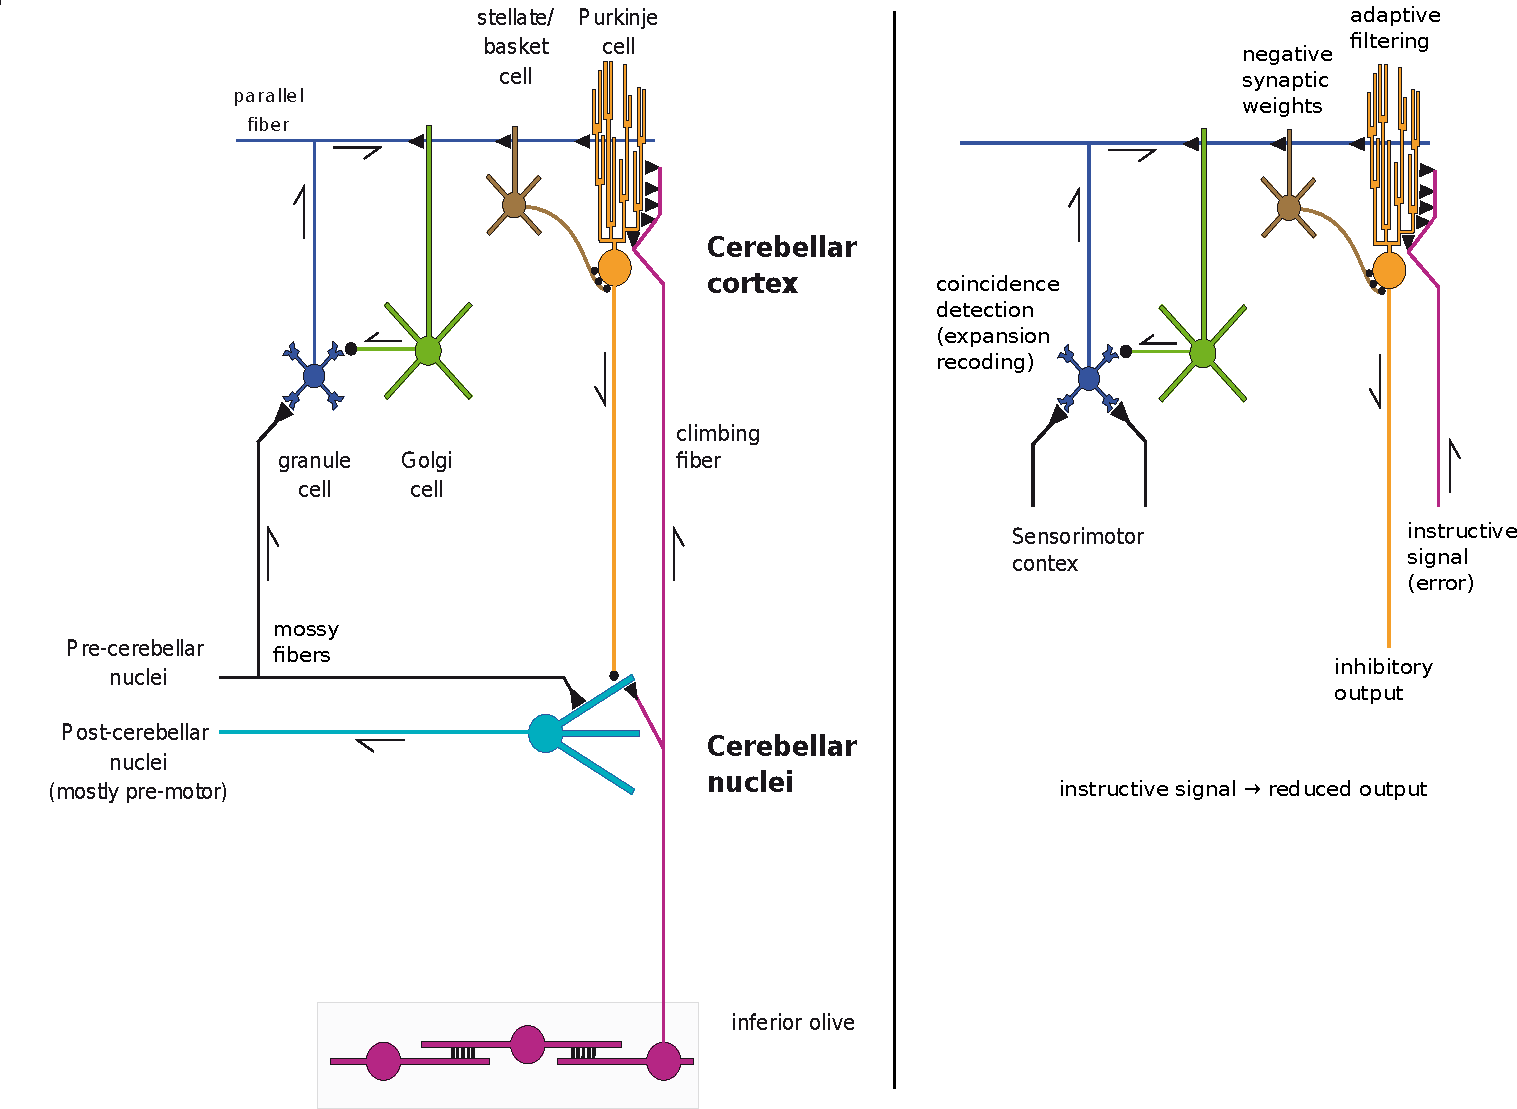
\includegraphics[scale=0.6]{anatomy.pdf}
			% \def\svgwidth{.3\textwidth}
			% \input{figures/anatomy.pdf_tex}
		  \caption{
		  \textbf{Anatomy and functionality of the cerebellar cortex}\\
		  The left figure is a simplified illustration of the anatomy of the cerebellar cortex. Inputs are sent to the cerebellum from the pre-cerebellar nuclei through mossy fibers (in black), and through the inferior olive (in purple). Both inputs make synapses in the cerebellar nuclei and in the cortex. In the cortex, climbing fibers are directly connected to the synaptic trees of Purkinje cells, while mossy fibers make first synapses with granule cells. Granule cell axons are called parallel fibers, and they are the main input of Purkinje cells. Some parallel fibers make first synapses with an interneuron, the stellate or the basket cells. 
	  In the right diagram it is shown the theorized function of each element of the cerebellar cortex. Mossy fibers bring the sensimotor cortex. Granule cells recode the signal, and interneurons allow negative weights between them and Purkinje cells. Purkinje cells apply the actual filtering, which is made adapted to the input through the instructive signal coming from the climbing fibers.}
		  \label{anatomy}}}
\end{figure}


This synaptic organization is repeated across the whole cerebellar cortex in an extremely modular fashion, where groups of Purkinje neurons form \emph{microzones} that share similar teaching signals and probably project to the same groups of cells in the deep cerebellar nuclei (DCN). The DCN neurons send their axons to many brain regions, and they contribute to many fundamental processes even outside the movement context, such as aversive learning \cite{frontera2020bidirectional}. Therefore, understanding how their activity is modulated is of utter importance for solving many crucial problems in neuroscience.

The mechanism through which Purkinje cells modulated the output of the DCN is still unclear. In fact, the traditional theory was the DCN neurons were activated by mossy fibers inputs and modulated by the inhibitory inputs from Purkinje cells. Furthermore, precise temporal coding of neural activity has been investigated mostly in the context of excitatory input, while an increased interest for the contribution of inhibitory inhibitory inputs to the rate and timing of DCN firing started at the beginning of the millennium \cite{person2012synchrony}. The hypothesis that we want to support with this experiment is that Purkinje cells exert control on DCN cells with a synchrony coding, as opposed to a rate coding. They would achieve that by sending many synchronous inhibitory signals to DCN neurons at all times where they should not fire, and letting open windows where the DCN neurons can fire by desynchronizing. This model would allow millisecond-scale temporal precision, and it has been already investigated in the past at the level of the DCN \cite{person2012synchrony}. Yet, to which extent Purkinje cells get synchronized during a task remain largely unexplored.

The objective of my project was to analyse electrophysiological data from my host lab to examine to which extent neighbor Purkinje cells (presumably belonging to the same microzone) and distant Purkinje cells are differentially synchronized in the course of periods of active recruitment.
My contribution to this project has been the implementation of the analyses of the data, along with a reproducible and open pipeline. I've achieved this using contemporary resources that I believe will contribute to the community of neuroscience, for example the use of Julia, a scientific oriented programming language that allowed me to maintain a clean, modular and reusable code base for the project. 

